% Options for packages loaded elsewhere
\PassOptionsToPackage{unicode}{hyperref}
\PassOptionsToPackage{hyphens}{url}
%
\documentclass[
]{article}
\usepackage{amsmath,amssymb}
\usepackage{lmodern}
\usepackage{iftex}
\ifPDFTeX
  \usepackage[T1]{fontenc}
  \usepackage[utf8]{inputenc}
  \usepackage{textcomp} % provide euro and other symbols
\else % if luatex or xetex
  \usepackage{unicode-math}
  \defaultfontfeatures{Scale=MatchLowercase}
  \defaultfontfeatures[\rmfamily]{Ligatures=TeX,Scale=1}
\fi
% Use upquote if available, for straight quotes in verbatim environments
\IfFileExists{upquote.sty}{\usepackage{upquote}}{}
\IfFileExists{microtype.sty}{% use microtype if available
  \usepackage[]{microtype}
  \UseMicrotypeSet[protrusion]{basicmath} % disable protrusion for tt fonts
}{}
\makeatletter
\@ifundefined{KOMAClassName}{% if non-KOMA class
  \IfFileExists{parskip.sty}{%
    \usepackage{parskip}
  }{% else
    \setlength{\parindent}{0pt}
    \setlength{\parskip}{6pt plus 2pt minus 1pt}}
}{% if KOMA class
  \KOMAoptions{parskip=half}}
\makeatother
\usepackage{xcolor}
\usepackage[margin=1in]{geometry}
\usepackage{color}
\usepackage{fancyvrb}
\newcommand{\VerbBar}{|}
\newcommand{\VERB}{\Verb[commandchars=\\\{\}]}
\DefineVerbatimEnvironment{Highlighting}{Verbatim}{commandchars=\\\{\}}
% Add ',fontsize=\small' for more characters per line
\usepackage{framed}
\definecolor{shadecolor}{RGB}{248,248,248}
\newenvironment{Shaded}{\begin{snugshade}}{\end{snugshade}}
\newcommand{\AlertTok}[1]{\textcolor[rgb]{0.94,0.16,0.16}{#1}}
\newcommand{\AnnotationTok}[1]{\textcolor[rgb]{0.56,0.35,0.01}{\textbf{\textit{#1}}}}
\newcommand{\AttributeTok}[1]{\textcolor[rgb]{0.77,0.63,0.00}{#1}}
\newcommand{\BaseNTok}[1]{\textcolor[rgb]{0.00,0.00,0.81}{#1}}
\newcommand{\BuiltInTok}[1]{#1}
\newcommand{\CharTok}[1]{\textcolor[rgb]{0.31,0.60,0.02}{#1}}
\newcommand{\CommentTok}[1]{\textcolor[rgb]{0.56,0.35,0.01}{\textit{#1}}}
\newcommand{\CommentVarTok}[1]{\textcolor[rgb]{0.56,0.35,0.01}{\textbf{\textit{#1}}}}
\newcommand{\ConstantTok}[1]{\textcolor[rgb]{0.00,0.00,0.00}{#1}}
\newcommand{\ControlFlowTok}[1]{\textcolor[rgb]{0.13,0.29,0.53}{\textbf{#1}}}
\newcommand{\DataTypeTok}[1]{\textcolor[rgb]{0.13,0.29,0.53}{#1}}
\newcommand{\DecValTok}[1]{\textcolor[rgb]{0.00,0.00,0.81}{#1}}
\newcommand{\DocumentationTok}[1]{\textcolor[rgb]{0.56,0.35,0.01}{\textbf{\textit{#1}}}}
\newcommand{\ErrorTok}[1]{\textcolor[rgb]{0.64,0.00,0.00}{\textbf{#1}}}
\newcommand{\ExtensionTok}[1]{#1}
\newcommand{\FloatTok}[1]{\textcolor[rgb]{0.00,0.00,0.81}{#1}}
\newcommand{\FunctionTok}[1]{\textcolor[rgb]{0.00,0.00,0.00}{#1}}
\newcommand{\ImportTok}[1]{#1}
\newcommand{\InformationTok}[1]{\textcolor[rgb]{0.56,0.35,0.01}{\textbf{\textit{#1}}}}
\newcommand{\KeywordTok}[1]{\textcolor[rgb]{0.13,0.29,0.53}{\textbf{#1}}}
\newcommand{\NormalTok}[1]{#1}
\newcommand{\OperatorTok}[1]{\textcolor[rgb]{0.81,0.36,0.00}{\textbf{#1}}}
\newcommand{\OtherTok}[1]{\textcolor[rgb]{0.56,0.35,0.01}{#1}}
\newcommand{\PreprocessorTok}[1]{\textcolor[rgb]{0.56,0.35,0.01}{\textit{#1}}}
\newcommand{\RegionMarkerTok}[1]{#1}
\newcommand{\SpecialCharTok}[1]{\textcolor[rgb]{0.00,0.00,0.00}{#1}}
\newcommand{\SpecialStringTok}[1]{\textcolor[rgb]{0.31,0.60,0.02}{#1}}
\newcommand{\StringTok}[1]{\textcolor[rgb]{0.31,0.60,0.02}{#1}}
\newcommand{\VariableTok}[1]{\textcolor[rgb]{0.00,0.00,0.00}{#1}}
\newcommand{\VerbatimStringTok}[1]{\textcolor[rgb]{0.31,0.60,0.02}{#1}}
\newcommand{\WarningTok}[1]{\textcolor[rgb]{0.56,0.35,0.01}{\textbf{\textit{#1}}}}
\usepackage{graphicx}
\makeatletter
\def\maxwidth{\ifdim\Gin@nat@width>\linewidth\linewidth\else\Gin@nat@width\fi}
\def\maxheight{\ifdim\Gin@nat@height>\textheight\textheight\else\Gin@nat@height\fi}
\makeatother
% Scale images if necessary, so that they will not overflow the page
% margins by default, and it is still possible to overwrite the defaults
% using explicit options in \includegraphics[width, height, ...]{}
\setkeys{Gin}{width=\maxwidth,height=\maxheight,keepaspectratio}
% Set default figure placement to htbp
\makeatletter
\def\fps@figure{htbp}
\makeatother
\setlength{\emergencystretch}{3em} % prevent overfull lines
\providecommand{\tightlist}{%
  \setlength{\itemsep}{0pt}\setlength{\parskip}{0pt}}
\setcounter{secnumdepth}{5}
\ifLuaTeX
  \usepackage{selnolig}  % disable illegal ligatures
\fi
\IfFileExists{bookmark.sty}{\usepackage{bookmark}}{\usepackage{hyperref}}
\IfFileExists{xurl.sty}{\usepackage{xurl}}{} % add URL line breaks if available
\urlstyle{same} % disable monospaced font for URLs
\hypersetup{
  pdftitle={V1075 Monte Carlo Report},
  hidelinks,
  pdfcreator={LaTeX via pandoc}}

\title{V1075 Monte Carlo Report}
\author{}
\date{\vspace{-2.5em}}

\begin{document}
\maketitle

{
\setcounter{tocdepth}{2}
\tableofcontents
}
\vspace{1em}
\begin{center}
\begin{minipage}{0.95\textwidth}
\setlength{\fboxsep}{10pt}
\noindent\colorbox{gray!10}{
  \parbox{\textwidth}{
    \textbf{\large Purpose:} This report performs Monte Carlo simulations to quantify uncertainty in estimates of $\delta^{18}$O$_{surface.water}$ ($\delta^{18}$O$_{sw}$) and paleotemperature derived from $\delta^{18}$O$_{phosphate}$ ($\delta^{18}$O$_{p}$) values of vertebrate fossils collected from the V1075 bonebed of the Cloverly Formation.

    \vspace{0.5em}

    \textbf{\large Structure:} The document includes steps for data loading, bootstrapping of $\delta^{18}$O$_{p}$, simulation of $\delta^{18}$O$_{sw}$ and paleotemperature distributions, and uncertainty quantification.

    \vspace{0.5em}

    \textbf{\large Reproducibility:}To run this report, open the associated RStudio Project file (\texttt{Frontiers\_V1075\_Project.Rproj}). This automatically sets the correct working directory. Then run this \texttt{.Rmd} file.

    \vspace{0.5em}

    \textbf{\large Repository:} All data and code used are provided at:
    \href{https://github.com/mattgeo1990/Frontiers-Allen-et-al.-2025/tree/main/Frontiers_V1075_Project}{\color{blue}\texttt{github.com/.../Frontiers\_V1075\_Project}}\\
    → Start by reading the \texttt{README.md} file in that directory.

    \vspace{0.5em}

    \textbf{\large Citation:} Allen et al., 2025. \textit{Frontiers in Earth Science}, DOI:\\
    \href{https://doi.org/10.3389/feart.2025.1497416}{10.3389/feart.2025.1497416}
  }
}
\end{minipage}
\end{center}
\vspace{2em}

\hypertarget{setup}{%
\section{Setup}\label{setup}}

\begin{Shaded}
\begin{Highlighting}[]
\CommentTok{\# Define directories using here::here()}
\CommentTok{\# Correct project{-}relative paths}
\NormalTok{data\_dir }\OtherTok{\textless{}{-}} \FunctionTok{here}\NormalTok{(}\StringTok{"data"}\NormalTok{)}
\NormalTok{results\_dir }\OtherTok{\textless{}{-}} \FunctionTok{here}\NormalTok{(}\StringTok{"results"}\NormalTok{)}
\NormalTok{models\_dir }\OtherTok{\textless{}{-}} \FunctionTok{here}\NormalTok{(}\StringTok{"models"}\NormalTok{)}

\CommentTok{\# Read in data}
\NormalTok{V1075\_MCdata }\OtherTok{\textless{}{-}} \FunctionTok{read\_csv}\NormalTok{(}\FunctionTok{file.path}\NormalTok{(data\_dir, }\StringTok{"V1075MC\_data.csv"}\NormalTok{))}
\NormalTok{NIST120c }\OtherTok{\textless{}{-}} \FunctionTok{read\_csv}\NormalTok{(}\FunctionTok{file.path}\NormalTok{(data\_dir, }\StringTok{"V1075\_NIST120c.csv"}\NormalTok{))}

\CommentTok{\# Load models using project{-}root{-}relative paths}
\NormalTok{Amiot\_lm }\OtherTok{\textless{}{-}} \FunctionTok{readRDS}\NormalTok{(}\FunctionTok{here}\NormalTok{(}\StringTok{"models"}\NormalTok{, }\StringTok{"Amiot\_reg\_lm.rds"}\NormalTok{))}
\NormalTok{Barrick\_lm }\OtherTok{\textless{}{-}} \FunctionTok{readRDS}\NormalTok{(}\FunctionTok{here}\NormalTok{(}\StringTok{"models"}\NormalTok{, }\StringTok{"Barrick\_reg\_lm.rds"}\NormalTok{))}
\NormalTok{PLN\_lm }\OtherTok{\textless{}{-}} \FunctionTok{readRDS}\NormalTok{(}\FunctionTok{here}\NormalTok{(}\StringTok{"models"}\NormalTok{, }\StringTok{"PLNd18Op\_reg\_lm.rds"}\NormalTok{))}
\NormalTok{TwTa\_lm }\OtherTok{\textless{}{-}} \FunctionTok{readRDS}\NormalTok{(}\FunctionTok{here}\NormalTok{(}\StringTok{"models"}\NormalTok{, }\StringTok{"TwTa\_reg\_lm.rds"}\NormalTok{))}

\CommentTok{\# Set constants}
\NormalTok{n\_iterations }\OtherTok{\textless{}{-}} \DecValTok{1000}
\FunctionTok{set.seed}\NormalTok{(}\DecValTok{123}\NormalTok{)}
\end{Highlighting}
\end{Shaded}

\hypertarget{bootstrapping}{%
\section{\texorpdfstring{Bootstrapping \(\delta^{18}O_{p}\) by
Taxon}{Bootstrapping \textbackslash delta\^{}\{18\}O\_\{p\} by Taxon}}\label{bootstrapping}}

\begin{Shaded}
\begin{Highlighting}[]
\CommentTok{\# Subset taxa into a list of vectors}
\NormalTok{taxa\_list }\OtherTok{\textless{}{-}} \FunctionTok{list}\NormalTok{(}
  \AttributeTok{Lepisosteidae       =} \FunctionTok{subset}\NormalTok{(V1075\_MCdata, Taxon }\SpecialCharTok{==} \StringTok{"Lepisosteids"}\NormalTok{)}\SpecialCharTok{$}\NormalTok{d18O,}
  \AttributeTok{Hybodontiformes     =} \FunctionTok{subset}\NormalTok{(V1075\_MCdata, Taxon }\SpecialCharTok{==} \StringTok{"Hybodonts"}\NormalTok{)}\SpecialCharTok{$}\NormalTok{d18O,}
  \StringTok{\textasciigrave{}}\AttributeTok{Glyptops sp.}\StringTok{\textasciigrave{}}      \OtherTok{=} \FunctionTok{subset}\NormalTok{(V1075\_MCdata, Taxon }\SpecialCharTok{==} \StringTok{"Glyptops sp."}\NormalTok{)}\SpecialCharTok{$}\NormalTok{d18O,}
  \StringTok{\textasciigrave{}}\AttributeTok{Naomichelys sp.}\StringTok{\textasciigrave{}}   \OtherTok{=} \FunctionTok{subset}\NormalTok{(V1075\_MCdata, Taxon }\SpecialCharTok{==} \StringTok{"Naomichelys sp."}\NormalTok{)}\SpecialCharTok{$}\NormalTok{d18O,}
  \StringTok{\textasciigrave{}}\AttributeTok{Neosuchian G}\StringTok{\textasciigrave{}}      \OtherTok{=} \FunctionTok{subset}\NormalTok{(V1075\_MCdata, Taxon }\SpecialCharTok{==} \StringTok{"Neosuchian G"}\NormalTok{)}\SpecialCharTok{$}\NormalTok{d18O,}
  \StringTok{\textasciigrave{}}\AttributeTok{Neosuchian A}\StringTok{\textasciigrave{}}      \OtherTok{=} \FunctionTok{subset}\NormalTok{(V1075\_MCdata, Taxon }\SpecialCharTok{==} \StringTok{"Neosuchian A"}\NormalTok{)}\SpecialCharTok{$}\NormalTok{d18O,}
  \StringTok{\textasciigrave{}}\AttributeTok{Neosuchian B}\StringTok{\textasciigrave{}}      \OtherTok{=} \FunctionTok{subset}\NormalTok{(V1075\_MCdata, Taxon }\SpecialCharTok{==} \StringTok{"Neosuchian B"}\NormalTok{)}\SpecialCharTok{$}\NormalTok{d18O,}
  \AttributeTok{NIST12Oc\_aka\_NBS120c =}\NormalTok{ NIST120c}\SpecialCharTok{$}\NormalTok{d}\FloatTok{.18}\NormalTok{O}\FloatTok{.16}\NormalTok{O}
\NormalTok{)}

\CommentTok{\# Define bootstrap function}
\NormalTok{taxon\_bootstrap }\OtherTok{\textless{}{-}} \ControlFlowTok{function}\NormalTok{(values) \{}
  \FunctionTok{data.frame}\NormalTok{(}\AttributeTok{means =} \FunctionTok{replicate}\NormalTok{(n\_iterations, }\FunctionTok{mean}\NormalTok{(}\FunctionTok{sample}\NormalTok{(values, }\AttributeTok{replace =} \ConstantTok{TRUE}\NormalTok{))))}
\NormalTok{\}}

\CommentTok{\# Apply bootstrap to each taxon}
\NormalTok{bootstrap\_results }\OtherTok{\textless{}{-}} \FunctionTok{lapply}\NormalTok{(taxa\_list, taxon\_bootstrap)}

\CommentTok{\# Name the results list for easy access}
\FunctionTok{names}\NormalTok{(bootstrap\_results) }\OtherTok{\textless{}{-}} \FunctionTok{names}\NormalTok{(taxa\_list)}

\NormalTok{bootstrap\_results }\OtherTok{\textless{}{-}} \FunctionTok{lapply}\NormalTok{(taxa\_list, taxon\_bootstrap)}

\CommentTok{\# Combine bootstrap data}
\NormalTok{combined\_data }\OtherTok{\textless{}{-}} \FunctionTok{bind\_rows}\NormalTok{(}
  \FunctionTok{lapply}\NormalTok{(}\FunctionTok{names}\NormalTok{(bootstrap\_results), }\ControlFlowTok{function}\NormalTok{(t) \{}
    \FunctionTok{tibble}\NormalTok{(}\AttributeTok{group =}\NormalTok{ t, }\AttributeTok{values =}\NormalTok{ bootstrap\_results[[t]]}\SpecialCharTok{$}\NormalTok{means)}
\NormalTok{  \})}
\NormalTok{)}

\CommentTok{\# Summarize d18Op}
\NormalTok{summary\_d18Op }\OtherTok{\textless{}{-}}\NormalTok{ combined\_data }\SpecialCharTok{\%\textgreater{}\%}
  \FunctionTok{group\_by}\NormalTok{(group) }\SpecialCharTok{\%\textgreater{}\%}
  \FunctionTok{summarise}\NormalTok{(}
    \AttributeTok{Mean\_d18Op =} \FunctionTok{mean}\NormalTok{(values),}
    \AttributeTok{CI\_Lower =} \FunctionTok{quantile}\NormalTok{(values, }\FloatTok{0.025}\NormalTok{, }\AttributeTok{na.rm =} \ConstantTok{TRUE}\NormalTok{),}
    \AttributeTok{CI\_Upper =} \FunctionTok{quantile}\NormalTok{(values, }\FloatTok{0.975}\NormalTok{, }\AttributeTok{na.rm =} \ConstantTok{TRUE}\NormalTok{)}
\NormalTok{  )}

\NormalTok{summary\_d18Op}
\end{Highlighting}
\end{Shaded}

\begin{verbatim}
## # A tibble: 8 x 4
##   group                Mean_d18Op CI_Lower CI_Upper
##   <chr>                     <dbl>    <dbl>    <dbl>
## 1 Glyptops sp.               13.8    12.6      14.9
## 2 Hybodontiformes            12.0     9.77     15.3
## 3 Lepisosteidae              13.8    13.0      14.5
## 4 NIST12Oc_aka_NBS120c       22.6    22.4      22.7
## 5 Naomichelys sp.            14.3    14.0      14.7
## 6 Neosuchian A               17.1    16.0      18.5
## 7 Neosuchian B               16.6    15.5      17.6
## 8 Neosuchian G               14.0    12.4      15.5
\end{verbatim}

\begin{Shaded}
\begin{Highlighting}[]
\CommentTok{\# Prepare to plot histogram of d18Op simulations}
\NormalTok{combined\_data}\SpecialCharTok{$}\NormalTok{group }\OtherTok{\textless{}{-}} \FunctionTok{factor}\NormalTok{(combined\_data}\SpecialCharTok{$}\NormalTok{group, }
  \AttributeTok{levels =} \FunctionTok{names}\NormalTok{(taxa\_list))}

\CommentTok{\# Plot}
\FunctionTok{ggplot}\NormalTok{(combined\_data, }\FunctionTok{aes}\NormalTok{(}\AttributeTok{x =}\NormalTok{ values, }\AttributeTok{fill =}\NormalTok{ group)) }\SpecialCharTok{+}
  \FunctionTok{geom\_histogram}\NormalTok{(}\AttributeTok{position =} \StringTok{"identity"}\NormalTok{, }\AttributeTok{alpha =} \FloatTok{0.7}\NormalTok{, }\AttributeTok{bins =} \DecValTok{30}\NormalTok{, }\AttributeTok{color =} \StringTok{"black"}\NormalTok{) }\SpecialCharTok{+}
  \FunctionTok{labs}\NormalTok{(}\AttributeTok{title =} \StringTok{"Histogram of Resampled Means"}\NormalTok{, }\AttributeTok{x =} \StringTok{"d18O\_p Values"}\NormalTok{, }\AttributeTok{y =} \StringTok{"Frequency"}\NormalTok{) }\SpecialCharTok{+}
  \FunctionTok{theme\_minimal}\NormalTok{() }\SpecialCharTok{+}
  \FunctionTok{facet\_wrap}\NormalTok{(}\SpecialCharTok{\textasciitilde{}}\NormalTok{group, }\AttributeTok{scales =} \StringTok{"free"}\NormalTok{)}
\end{Highlighting}
\end{Shaded}

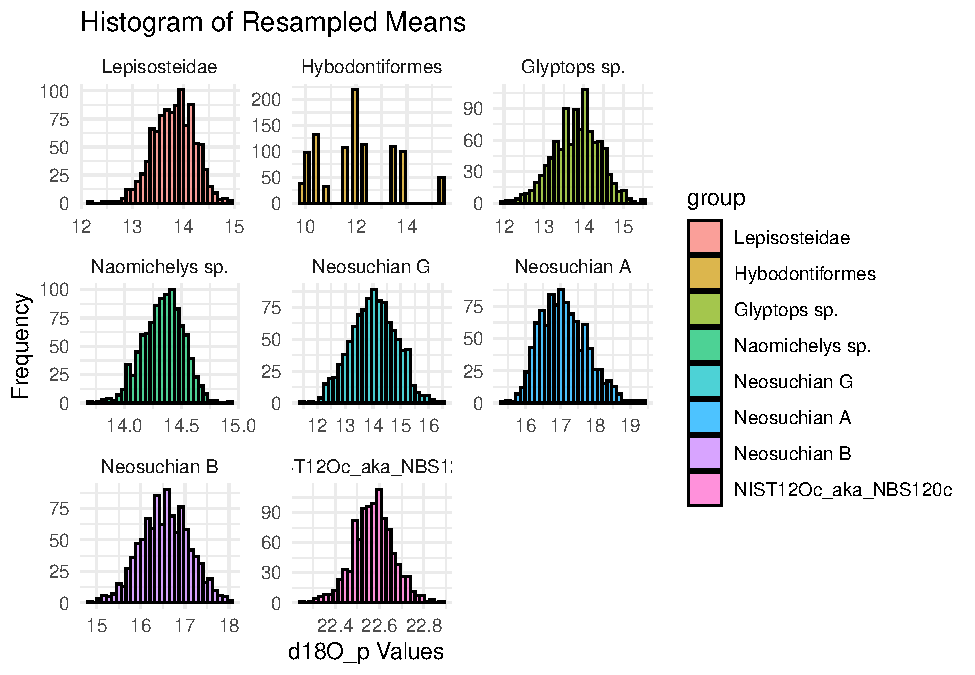
\includegraphics{V1075_MonteCarlo_Report_files/figure-latex/unnamed-chunk-2-1.pdf}

\hypertarget{d18Osw_simulation}{%
\section{\texorpdfstring{Water \(\delta^{18}O_{sw}\)
Simulations}{Water \textbackslash delta\^{}\{18\}O\_\{sw\} Simulations}}\label{d18Osw_simulation}}

\begin{Shaded}
\begin{Highlighting}[]
\CommentTok{\# Create d18Osw simulation function}
\NormalTok{simulate\_water }\OtherTok{\textless{}{-}} \ControlFlowTok{function}\NormalTok{(means\_vector, model) \{}
\NormalTok{  intercept\_sim }\OtherTok{\textless{}{-}} \FunctionTok{rnorm}\NormalTok{(n\_iterations, }\AttributeTok{mean =} \FunctionTok{coef}\NormalTok{(model)[}\DecValTok{1}\NormalTok{], }\AttributeTok{sd =} \FunctionTok{summary}\NormalTok{(model)}\SpecialCharTok{$}\NormalTok{coefficients[}\DecValTok{1}\NormalTok{,}\DecValTok{2}\NormalTok{])}
\NormalTok{  slope\_sim }\OtherTok{\textless{}{-}} \FunctionTok{rnorm}\NormalTok{(n\_iterations, }\AttributeTok{mean =} \FunctionTok{coef}\NormalTok{(model)[}\DecValTok{2}\NormalTok{], }\AttributeTok{sd =} \FunctionTok{summary}\NormalTok{(model)}\SpecialCharTok{$}\NormalTok{coefficients[}\DecValTok{2}\NormalTok{,}\DecValTok{2}\NormalTok{])}
\NormalTok{  residuals\_sim }\OtherTok{\textless{}{-}} \FunctionTok{rnorm}\NormalTok{(n\_iterations, }\AttributeTok{mean =} \DecValTok{0}\NormalTok{, }\AttributeTok{sd =} \FunctionTok{summary}\NormalTok{(model)}\SpecialCharTok{$}\NormalTok{sigma)}
  
  \FunctionTok{rep}\NormalTok{(means\_vector, }\AttributeTok{each =}\NormalTok{ n\_iterations) }\SpecialCharTok{*} \FunctionTok{rep}\NormalTok{(slope\_sim, }\AttributeTok{times =} \FunctionTok{length}\NormalTok{(means\_vector)) }\SpecialCharTok{+}
    \FunctionTok{rep}\NormalTok{(intercept\_sim, }\AttributeTok{times =} \FunctionTok{length}\NormalTok{(means\_vector)) }\SpecialCharTok{+}
    \FunctionTok{rep}\NormalTok{(residuals\_sim, }\AttributeTok{times =} \FunctionTok{length}\NormalTok{(means\_vector))}
\NormalTok{\}}

\CommentTok{\# List of target taxa and corresponding regression models}
\NormalTok{water\_sim\_targets }\OtherTok{\textless{}{-}} \FunctionTok{list}\NormalTok{(}
  \StringTok{"Glyptops sp."} \OtherTok{=}\NormalTok{ Barrick\_lm,    }\CommentTok{\# turtles {-}\textgreater{} Barrick regression}
  \StringTok{"Naomichelys sp."} \OtherTok{=}\NormalTok{ Barrick\_lm, }\CommentTok{\# turtles {-}\textgreater{} Barrick regression}
  \StringTok{"Neosuchian G"} \OtherTok{=}\NormalTok{ Amiot\_lm,      }\CommentTok{\# crocs {-}\textgreater{} Amiot regression}
  \StringTok{"Neosuchian A"} \OtherTok{=}\NormalTok{ Amiot\_lm,      }\CommentTok{\# crocs {-}\textgreater{} Amiot regression}
  \StringTok{"Neosuchian B"} \OtherTok{=}\NormalTok{ Amiot\_lm       }\CommentTok{\# crocs {-}\textgreater{} Amiot regression}
\NormalTok{)}

\CommentTok{\# Initialize a list to store results}
\NormalTok{water\_sim\_results }\OtherTok{\textless{}{-}} \FunctionTok{list}\NormalTok{()}

\CommentTok{\# Initialize list to store full simulated distributions}
\NormalTok{water\_sim\_distributions }\OtherTok{\textless{}{-}} \FunctionTok{list}\NormalTok{()}

\CommentTok{\# Loop over each target taxon}
\FunctionTok{set.seed}\NormalTok{(}\DecValTok{123}\NormalTok{)}
\ControlFlowTok{for}\NormalTok{ (taxon }\ControlFlowTok{in} \FunctionTok{names}\NormalTok{(water\_sim\_targets)) \{}
\NormalTok{  sim\_result }\OtherTok{\textless{}{-}} \FunctionTok{simulate\_water}\NormalTok{(bootstrap\_results[[taxon]]}\SpecialCharTok{$}\NormalTok{means, water\_sim\_targets[[taxon]])}
  
  \CommentTok{\# Save summary results}
\NormalTok{  water\_sim\_results[[taxon]] }\OtherTok{\textless{}{-}} \FunctionTok{list}\NormalTok{(}
    \AttributeTok{mean =} \FunctionTok{mean}\NormalTok{(sim\_result),}
    \AttributeTok{ci =} \FunctionTok{quantile}\NormalTok{(sim\_result, }\AttributeTok{probs =} \FunctionTok{c}\NormalTok{(}\FloatTok{0.025}\NormalTok{, }\FloatTok{0.975}\NormalTok{))}
\NormalTok{  )}
  
  \CommentTok{\# Save full distribution}
\NormalTok{  water\_sim\_distributions[[taxon]] }\OtherTok{\textless{}{-}}\NormalTok{ sim\_result}
  
  \CommentTok{\# Print summary results}
  \FunctionTok{cat}\NormalTok{(}\StringTok{"}\SpecialCharTok{\textbackslash{}n}\StringTok{"}\NormalTok{, taxon, }\StringTok{"Water Mean:"}\NormalTok{, }\FunctionTok{round}\NormalTok{(water\_sim\_results[[taxon]]}\SpecialCharTok{$}\NormalTok{mean, }\DecValTok{2}\NormalTok{))}
  \FunctionTok{cat}\NormalTok{(}\StringTok{"}\SpecialCharTok{\textbackslash{}n}\StringTok{95\% CI:"}\NormalTok{, }\FunctionTok{round}\NormalTok{(water\_sim\_results[[taxon]]}\SpecialCharTok{$}\NormalTok{ci, }\DecValTok{2}\NormalTok{), }\StringTok{"}\SpecialCharTok{\textbackslash{}n}\StringTok{"}\NormalTok{)}
\NormalTok{\}}
\end{Highlighting}
\end{Shaded}

\begin{verbatim}
## 
##  Glyptops sp. Water Mean: -8.29
## 95% CI: -10.52 -5.95 
## 
##  Naomichelys sp. Water Mean: -7.77
## 95% CI: -9.81 -5.8 
## 
##  Neosuchian G Water Mean: -7.6
## 95% CI: -11.4 -3.67 
## 
##  Neosuchian A Water Mean: -5.06
## 95% CI: -8.76 -1.17 
## 
##  Neosuchian B Water Mean: -5.52
## 95% CI: -9.32 -1.91
\end{verbatim}

\begin{Shaded}
\begin{Highlighting}[]
\CommentTok{\# Simulate single d18Ow distribution based on crocG and Glyptops d18Ow}
\NormalTok{bootstrapped\_d18Ow }\OtherTok{\textless{}{-}} \FunctionTok{replicate}\NormalTok{(n\_iterations, \{}
\NormalTok{  sample\_glyp }\OtherTok{\textless{}{-}} \FunctionTok{sample}\NormalTok{(water\_sim\_distributions[[}\StringTok{"Glyptops sp."}\NormalTok{]], }\AttributeTok{size =} \DecValTok{1}\NormalTok{, }\AttributeTok{replace =} \ConstantTok{TRUE}\NormalTok{)}
\NormalTok{  sample\_crocG }\OtherTok{\textless{}{-}} \FunctionTok{sample}\NormalTok{(water\_sim\_distributions[[}\StringTok{"Neosuchian G"}\NormalTok{]], }\AttributeTok{size =} \DecValTok{1}\NormalTok{, }\AttributeTok{replace =} \ConstantTok{TRUE}\NormalTok{)}
  \FunctionTok{mean}\NormalTok{(}\FunctionTok{c}\NormalTok{(sample\_glyp, sample\_crocG))  }\CommentTok{\# Average of the two}
\NormalTok{\})}

\CommentTok{\# Analyze combined distribution}
\NormalTok{mean\_d18Ow }\OtherTok{\textless{}{-}} \FunctionTok{mean}\NormalTok{(bootstrapped\_d18Ow)}
\NormalTok{sd\_d18Ow }\OtherTok{\textless{}{-}} \FunctionTok{sd}\NormalTok{(bootstrapped\_d18Ow)}
\NormalTok{quantiles }\OtherTok{\textless{}{-}} \FunctionTok{quantile}\NormalTok{(bootstrapped\_d18Ow, }\AttributeTok{probs =} \FunctionTok{c}\NormalTok{(}\FloatTok{0.025}\NormalTok{, }\FloatTok{0.975}\NormalTok{))}

\NormalTok{mean\_alld18Owater\_synth }\OtherTok{\textless{}{-}}\NormalTok{ mean\_d18Ow}
\NormalTok{alld18Owater\_lower }\OtherTok{\textless{}{-}}\NormalTok{ quantiles[}\DecValTok{1}\NormalTok{]}
\NormalTok{alld18Owater\_upper }\OtherTok{\textless{}{-}}\NormalTok{ quantiles[}\DecValTok{2}\NormalTok{]}

\CommentTok{\# Print results}
\FunctionTok{cat}\NormalTok{(}\FunctionTok{paste0}\NormalTok{(}\StringTok{"Mean $}\SpecialCharTok{\textbackslash{}\textbackslash{}}\StringTok{delta\^{}\{18\}O\_\{w\}$: "}\NormalTok{, }\FunctionTok{round}\NormalTok{(mean\_d18Ow, }\DecValTok{2}\NormalTok{), }\StringTok{"}\SpecialCharTok{\textbackslash{}n}\StringTok{"}\NormalTok{))}
\end{Highlighting}
\end{Shaded}

\begin{verbatim}
## Mean $\delta^{18}O_{w}$: -7.9
\end{verbatim}

\begin{Shaded}
\begin{Highlighting}[]
\FunctionTok{cat}\NormalTok{(}\FunctionTok{paste0}\NormalTok{(}\StringTok{"95}\SpecialCharTok{\textbackslash{}\textbackslash{}}\StringTok{\% CI for $}\SpecialCharTok{\textbackslash{}\textbackslash{}}\StringTok{delta\^{}\{18\}O\_\{w\}$: ["}\NormalTok{, }\FunctionTok{round}\NormalTok{(quantiles[}\DecValTok{1}\NormalTok{], }\DecValTok{2}\NormalTok{), }\StringTok{", "}\NormalTok{, }\FunctionTok{round}\NormalTok{(quantiles[}\DecValTok{2}\NormalTok{], }\DecValTok{2}\NormalTok{), }\StringTok{"]}\SpecialCharTok{\textbackslash{}n}\StringTok{"}\NormalTok{))}
\end{Highlighting}
\end{Shaded}

\begin{verbatim}
## 95\% CI for $\delta^{18}O_{w}$: [-10.03, -5.77]
\end{verbatim}

\begin{Shaded}
\begin{Highlighting}[]
\NormalTok{mean\_alld18Owater\_synth }\OtherTok{\textless{}{-}}\NormalTok{ mean\_d18Ow}
\NormalTok{alld18Owater\_lower }\OtherTok{\textless{}{-}}\NormalTok{ quantiles[}\DecValTok{1}\NormalTok{]}
\NormalTok{alld18Owater\_upper }\OtherTok{\textless{}{-}}\NormalTok{ quantiles[}\DecValTok{2}\NormalTok{]}

\CommentTok{\# Plot d18Osw Histogram}
\CommentTok{\# Compute y{-}axis range for label placement}
\NormalTok{temp\_plot }\OtherTok{\textless{}{-}} \FunctionTok{ggplot}\NormalTok{(}\FunctionTok{data.frame}\NormalTok{(}\AttributeTok{d18Ow =}\NormalTok{ bootstrapped\_d18Ow), }\FunctionTok{aes}\NormalTok{(}\AttributeTok{x =}\NormalTok{ d18Ow)) }\SpecialCharTok{+}
  \FunctionTok{geom\_histogram}\NormalTok{(}\AttributeTok{bins =} \DecValTok{50}\NormalTok{)}
\NormalTok{y\_max }\OtherTok{\textless{}{-}} \FunctionTok{max}\NormalTok{(}\FunctionTok{ggplot\_build}\NormalTok{(temp\_plot)}\SpecialCharTok{$}\NormalTok{data[[}\DecValTok{1}\NormalTok{]]}\SpecialCharTok{$}\NormalTok{count)}
\NormalTok{buffer }\OtherTok{\textless{}{-}}\NormalTok{ y\_max }\SpecialCharTok{*} \FloatTok{0.1}
\NormalTok{label\_y }\OtherTok{\textless{}{-}}\NormalTok{ y\_max }\SpecialCharTok{+}\NormalTok{ buffer}

\CommentTok{\# Generate plot}
\FunctionTok{ggplot}\NormalTok{(}\FunctionTok{data.frame}\NormalTok{(}\AttributeTok{d18Ow =}\NormalTok{ bootstrapped\_d18Ow), }\FunctionTok{aes}\NormalTok{(}\AttributeTok{x =}\NormalTok{ d18Ow)) }\SpecialCharTok{+}
  \FunctionTok{geom\_histogram}\NormalTok{(}\AttributeTok{fill =} \StringTok{"skyblue"}\NormalTok{, }\AttributeTok{color =} \StringTok{"black"}\NormalTok{, }\AttributeTok{bins =} \DecValTok{50}\NormalTok{) }\SpecialCharTok{+}
  \FunctionTok{geom\_vline}\NormalTok{(}\AttributeTok{xintercept =}\NormalTok{ mean\_alld18Owater\_synth, }\AttributeTok{color =} \StringTok{"red"}\NormalTok{, }\AttributeTok{linetype =} \StringTok{"dashed"}\NormalTok{) }\SpecialCharTok{+}
  \FunctionTok{geom\_vline}\NormalTok{(}\AttributeTok{xintercept =} \FunctionTok{c}\NormalTok{(alld18Owater\_lower, alld18Owater\_upper), }\AttributeTok{color =} \StringTok{"blue"}\NormalTok{, }\AttributeTok{linetype =} \StringTok{"dotted"}\NormalTok{) }\SpecialCharTok{+}
  \FunctionTok{annotate}\NormalTok{(}\StringTok{"text"}\NormalTok{, }\AttributeTok{x =}\NormalTok{ mean\_alld18Owater\_synth, }\AttributeTok{y =}\NormalTok{ label\_y,}
           \AttributeTok{label =} \FunctionTok{paste}\NormalTok{(}\StringTok{"Mean ="}\NormalTok{, }\FunctionTok{round}\NormalTok{(mean\_alld18Owater\_synth, }\DecValTok{2}\NormalTok{)),}
           \AttributeTok{vjust =} \DecValTok{0}\NormalTok{, }\AttributeTok{color =} \StringTok{"red"}\NormalTok{, }\AttributeTok{size =} \FloatTok{3.5}\NormalTok{) }\SpecialCharTok{+}
  \FunctionTok{annotate}\NormalTok{(}\StringTok{"text"}\NormalTok{, }\AttributeTok{x =}\NormalTok{ alld18Owater\_lower, }\AttributeTok{y =}\NormalTok{ label\_y,}
           \AttributeTok{label =} \FunctionTok{paste}\NormalTok{(}\StringTok{"Lower 95\% CI ="}\NormalTok{, }\FunctionTok{round}\NormalTok{(alld18Owater\_lower, }\DecValTok{2}\NormalTok{)),}
           \AttributeTok{vjust =} \DecValTok{0}\NormalTok{, }\AttributeTok{color =} \StringTok{"blue"}\NormalTok{, }\AttributeTok{size =} \FloatTok{3.5}\NormalTok{, }\AttributeTok{hjust =} \FloatTok{1.1}\NormalTok{) }\SpecialCharTok{+}
  \FunctionTok{annotate}\NormalTok{(}\StringTok{"text"}\NormalTok{, }\AttributeTok{x =}\NormalTok{ alld18Owater\_upper, }\AttributeTok{y =}\NormalTok{ label\_y,}
           \AttributeTok{label =} \FunctionTok{paste}\NormalTok{(}\StringTok{"Upper 95\% CI ="}\NormalTok{, }\FunctionTok{round}\NormalTok{(alld18Owater\_upper, }\DecValTok{2}\NormalTok{)),}
           \AttributeTok{vjust =} \DecValTok{0}\NormalTok{, }\AttributeTok{color =} \StringTok{"blue"}\NormalTok{, }\AttributeTok{size =} \FloatTok{3.5}\NormalTok{, }\AttributeTok{hjust =} \SpecialCharTok{{-}}\FloatTok{0.1}\NormalTok{) }\SpecialCharTok{+}
  \FunctionTok{ylim}\NormalTok{(}\DecValTok{0}\NormalTok{, label\_y }\SpecialCharTok{*} \FloatTok{1.1}\NormalTok{) }\SpecialCharTok{+}
  \FunctionTok{labs}\NormalTok{(}
    \AttributeTok{title =} \FunctionTok{expression}\NormalTok{(}\StringTok{"Simulated "}\SpecialCharTok{*}\NormalTok{delta}\SpecialCharTok{\^{}}\DecValTok{18}\SpecialCharTok{*}\StringTok{"O"}\NormalTok{[sw]}\SpecialCharTok{*}\StringTok{" distribution"}\NormalTok{),}
    \AttributeTok{x =} \FunctionTok{expression}\NormalTok{(delta}\SpecialCharTok{\^{}}\DecValTok{18}\SpecialCharTok{*}\StringTok{"O"}\NormalTok{[sw]}\SpecialCharTok{*}\StringTok{" (permil VSMOW)"}\NormalTok{),}
    \AttributeTok{y =} \StringTok{"Count"}
\NormalTok{  ) }\SpecialCharTok{+}
  \FunctionTok{theme\_minimal}\NormalTok{()}
\end{Highlighting}
\end{Shaded}

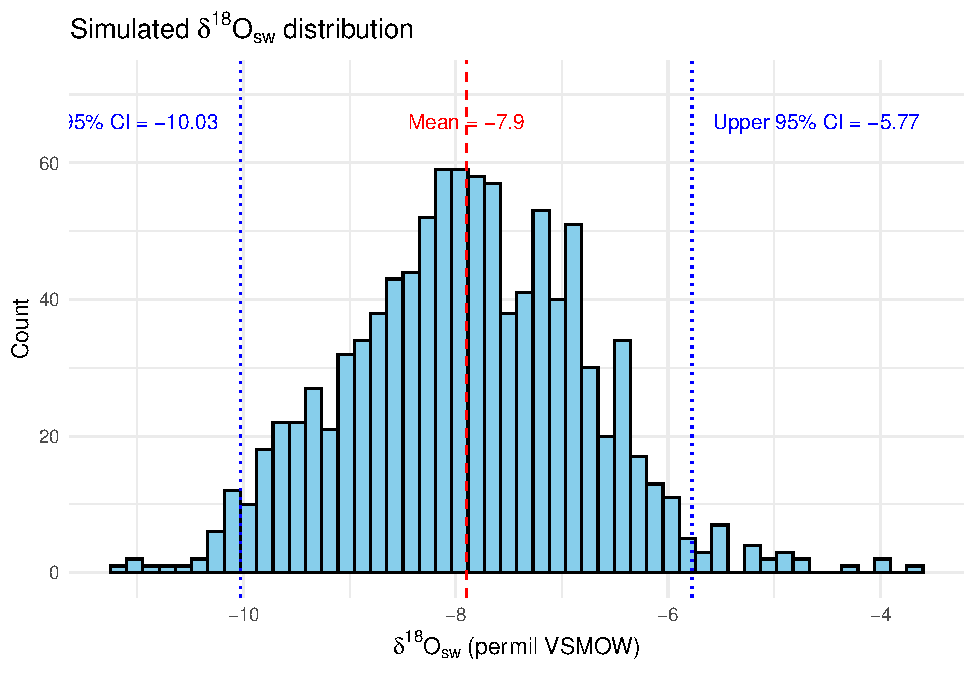
\includegraphics{V1075_MonteCarlo_Report_files/figure-latex/unnamed-chunk-3-1.pdf}

\begin{Shaded}
\begin{Highlighting}[]
\FunctionTok{ggsave}\NormalTok{(}\FunctionTok{file.path}\NormalTok{(results\_dir, }\StringTok{"d18Osw\_Histogram.png"}\NormalTok{))}
\end{Highlighting}
\end{Shaded}

\hypertarget{water_temperature_simulations}{%
\section{Water Temperature
Simulations}\label{water_temperature_simulations}}

\begin{Shaded}
\begin{Highlighting}[]
\NormalTok{delta\_Op }\OtherTok{\textless{}{-}}\NormalTok{ combined\_data}\SpecialCharTok{$}\NormalTok{values[combined\_data}\SpecialCharTok{$}\NormalTok{group }\SpecialCharTok{==} \StringTok{"Lepisosteidae"}\NormalTok{]}
\NormalTok{delta\_Ow }\OtherTok{\textless{}{-}}\NormalTok{ bootstrapped\_d18Ow}
\NormalTok{NIST\_sim }\OtherTok{\textless{}{-}}\NormalTok{ combined\_data}\SpecialCharTok{$}\NormalTok{values[combined\_data}\SpecialCharTok{$}\NormalTok{group }\SpecialCharTok{==} \StringTok{"NIST12Oc\_aka\_NBS120c"}\NormalTok{]}

\CommentTok{\# Simulate intercepts and slopes separately}
\NormalTok{intercept\_sim }\OtherTok{\textless{}{-}} \FunctionTok{rnorm}\NormalTok{(n\_iterations, }\AttributeTok{mean =} \FunctionTok{coef}\NormalTok{(PLN\_lm)[}\DecValTok{1}\NormalTok{], }\AttributeTok{sd =} \FunctionTok{summary}\NormalTok{(PLN\_lm)}\SpecialCharTok{$}\NormalTok{coefficients[}\DecValTok{1}\NormalTok{,}\DecValTok{2}\NormalTok{])}
\NormalTok{slope\_sim }\OtherTok{\textless{}{-}} \FunctionTok{rnorm}\NormalTok{(n\_iterations, }\AttributeTok{mean =} \FunctionTok{coef}\NormalTok{(PLN\_lm)[}\DecValTok{2}\NormalTok{], }\AttributeTok{sd =} \FunctionTok{summary}\NormalTok{(PLN\_lm)}\SpecialCharTok{$}\NormalTok{coefficients[}\DecValTok{2}\NormalTok{,}\DecValTok{2}\NormalTok{])}

\CommentTok{\# Simulate residuals}
\NormalTok{residual\_sim }\OtherTok{\textless{}{-}} \FunctionTok{rnorm}\NormalTok{(n\_iterations, }\AttributeTok{mean =} \DecValTok{0}\NormalTok{, }\AttributeTok{sd =} \FunctionTok{summary}\NormalTok{(PLN\_lm)}\SpecialCharTok{$}\NormalTok{sigma)}

\CommentTok{\# Now compute Tw\_simulations properly}
\FunctionTok{set.seed}\NormalTok{(}\DecValTok{123}\NormalTok{)}
\NormalTok{Tw\_simulations }\OtherTok{\textless{}{-}}\NormalTok{ intercept\_sim }\SpecialCharTok{+} 
\NormalTok{  slope\_sim }\SpecialCharTok{*}\NormalTok{ (delta\_Op }\SpecialCharTok{+}\NormalTok{ (}\FloatTok{22.6} \SpecialCharTok{{-}}\NormalTok{ NIST\_sim) }\SpecialCharTok{{-}}\NormalTok{ delta\_Ow) }\SpecialCharTok{+} 
\NormalTok{  residual\_sim}

\NormalTok{mean\_Tw }\OtherTok{\textless{}{-}} \FunctionTok{mean}\NormalTok{(Tw\_simulations)}
\NormalTok{ci\_Tw }\OtherTok{\textless{}{-}} \FunctionTok{quantile}\NormalTok{(Tw\_simulations, }\AttributeTok{probs =} \FunctionTok{c}\NormalTok{(}\FloatTok{0.025}\NormalTok{, }\FloatTok{0.975}\NormalTok{), }\AttributeTok{na.rm =} \ConstantTok{TRUE}\NormalTok{)}

\FunctionTok{cat}\NormalTok{(}\StringTok{"}\SpecialCharTok{\textbackslash{}n}\StringTok{Water Temperature Mean:"}\NormalTok{, mean\_Tw)}
\end{Highlighting}
\end{Shaded}

\begin{verbatim}
## 
## Water Temperature Mean: 26.00227
\end{verbatim}

\begin{Shaded}
\begin{Highlighting}[]
\FunctionTok{cat}\NormalTok{(}\StringTok{"}\SpecialCharTok{\textbackslash{}n}\StringTok{95\% CI:"}\NormalTok{, ci\_Tw, }\StringTok{"}\SpecialCharTok{\textbackslash{}n}\StringTok{"}\NormalTok{)}
\end{Highlighting}
\end{Shaded}

\begin{verbatim}
## 
## 95% CI: 8.864743 42.56411
\end{verbatim}

\begin{Shaded}
\begin{Highlighting}[]
\CommentTok{\# Plot Tw histogram}
\CommentTok{\# Calculate max y{-}value for adjustment (temporary plot to get y)}
\NormalTok{temp\_plot }\OtherTok{\textless{}{-}} \FunctionTok{ggplot}\NormalTok{(}\FunctionTok{data.frame}\NormalTok{(}\AttributeTok{Tw =}\NormalTok{ Tw\_simulations), }\FunctionTok{aes}\NormalTok{(}\AttributeTok{x =}\NormalTok{ Tw)) }\SpecialCharTok{+}
  \FunctionTok{geom\_histogram}\NormalTok{(}\AttributeTok{bins =} \DecValTok{50}\NormalTok{)}
\NormalTok{y\_max }\OtherTok{\textless{}{-}} \FunctionTok{ggplot\_build}\NormalTok{(temp\_plot)}\SpecialCharTok{$}\NormalTok{data[[}\DecValTok{1}\NormalTok{]]}\SpecialCharTok{$}\NormalTok{count }\SpecialCharTok{\%\textgreater{}\%} \FunctionTok{max}\NormalTok{()}

\CommentTok{\# Add 10\% headroom above max y{-}value for labels}
\NormalTok{buffer }\OtherTok{\textless{}{-}}\NormalTok{ y\_max }\SpecialCharTok{*} \FloatTok{0.1}
\NormalTok{label\_y }\OtherTok{\textless{}{-}}\NormalTok{ y\_max }\SpecialCharTok{+}\NormalTok{ buffer}

\CommentTok{\# Final plot with labels and spacing}
\FunctionTok{ggplot}\NormalTok{(}\FunctionTok{data.frame}\NormalTok{(}\AttributeTok{Tw =}\NormalTok{ Tw\_simulations), }\FunctionTok{aes}\NormalTok{(}\AttributeTok{x =}\NormalTok{ Tw)) }\SpecialCharTok{+}
  \FunctionTok{geom\_histogram}\NormalTok{(}\AttributeTok{fill =} \StringTok{"skyblue"}\NormalTok{, }\AttributeTok{color =} \StringTok{"black"}\NormalTok{, }\AttributeTok{bins =} \DecValTok{50}\NormalTok{) }\SpecialCharTok{+}
  \FunctionTok{geom\_vline}\NormalTok{(}\AttributeTok{xintercept =}\NormalTok{ mean\_Tw, }\AttributeTok{color =} \StringTok{"red"}\NormalTok{, }\AttributeTok{linetype =} \StringTok{"dashed"}\NormalTok{) }\SpecialCharTok{+}
  \FunctionTok{geom\_vline}\NormalTok{(}\AttributeTok{xintercept =}\NormalTok{ ci\_Tw, }\AttributeTok{color =} \StringTok{"blue"}\NormalTok{, }\AttributeTok{linetype =} \StringTok{"dotted"}\NormalTok{) }\SpecialCharTok{+}
  \FunctionTok{annotate}\NormalTok{(}\StringTok{"text"}\NormalTok{, }\AttributeTok{x =}\NormalTok{ mean\_Tw, }\AttributeTok{y =}\NormalTok{ label\_y, }\AttributeTok{label =} \FunctionTok{paste0}\NormalTok{(}\StringTok{"Mean = "}\NormalTok{, }\FunctionTok{round}\NormalTok{(mean\_Tw, }\DecValTok{2}\NormalTok{)),}
           \AttributeTok{vjust =} \DecValTok{0}\NormalTok{, }\AttributeTok{color =} \StringTok{"red"}\NormalTok{, }\AttributeTok{size =} \FloatTok{3.5}\NormalTok{) }\SpecialCharTok{+}
  \FunctionTok{annotate}\NormalTok{(}\StringTok{"text"}\NormalTok{, }\AttributeTok{x =}\NormalTok{ ci\_Tw[}\DecValTok{1}\NormalTok{], }\AttributeTok{y =}\NormalTok{ label\_y, }\AttributeTok{label =} \FunctionTok{paste0}\NormalTok{(}\StringTok{"Lower 95\% CI = "}\NormalTok{, }\FunctionTok{round}\NormalTok{(ci\_Tw[}\DecValTok{1}\NormalTok{], }\DecValTok{2}\NormalTok{)),}
           \AttributeTok{vjust =} \DecValTok{0}\NormalTok{, }\AttributeTok{color =} \StringTok{"blue"}\NormalTok{, }\AttributeTok{size =} \FloatTok{3.5}\NormalTok{) }\SpecialCharTok{+}
  \FunctionTok{annotate}\NormalTok{(}\StringTok{"text"}\NormalTok{, }\AttributeTok{x =}\NormalTok{ ci\_Tw[}\DecValTok{2}\NormalTok{], }\AttributeTok{y =}\NormalTok{ label\_y, }\AttributeTok{label =} \FunctionTok{paste0}\NormalTok{(}\StringTok{"Upper 95\% CI = "}\NormalTok{, }\FunctionTok{round}\NormalTok{(ci\_Tw[}\DecValTok{2}\NormalTok{], }\DecValTok{2}\NormalTok{)),}
           \AttributeTok{vjust =} \DecValTok{0}\NormalTok{, }\AttributeTok{color =} \StringTok{"blue"}\NormalTok{, }\AttributeTok{size =} \FloatTok{3.5}\NormalTok{) }\SpecialCharTok{+}
  \FunctionTok{ylim}\NormalTok{(}\DecValTok{0}\NormalTok{, label\_y }\SpecialCharTok{*} \FloatTok{1.1}\NormalTok{) }\SpecialCharTok{+}
  \FunctionTok{labs}\NormalTok{(}\AttributeTok{title =} \StringTok{"Simulated Water Temperature (Tw)"}\NormalTok{,}
       \AttributeTok{x =} \StringTok{"Water Temp (°C)"}\NormalTok{, }\AttributeTok{y =} \StringTok{"Count"}\NormalTok{) }\SpecialCharTok{+}
  \FunctionTok{theme\_minimal}\NormalTok{()}
\end{Highlighting}
\end{Shaded}

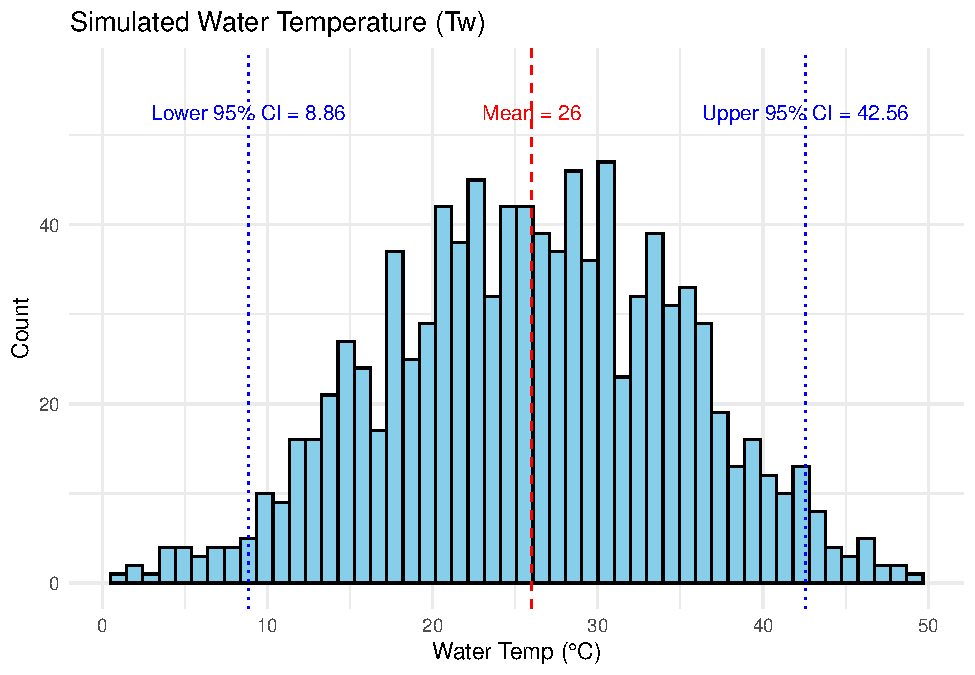
\includegraphics{V1075_MonteCarlo_Report_files/figure-latex/unnamed-chunk-4-1.pdf}

\begin{Shaded}
\begin{Highlighting}[]
\FunctionTok{ggsave}\NormalTok{(}\FunctionTok{file.path}\NormalTok{(results\_dir, }\StringTok{"Tw\_Histogram.png"}\NormalTok{))}
\end{Highlighting}
\end{Shaded}

\hypertarget{air_temperature_simulations}{%
\section{Air Temperature
Simulations}\label{air_temperature_simulations}}

\begin{Shaded}
\begin{Highlighting}[]
\CommentTok{\# Simulate intercept and slope}
\NormalTok{intercept\_sim }\OtherTok{\textless{}{-}} \FunctionTok{rnorm}\NormalTok{(n\_iterations, }\AttributeTok{mean =} \FunctionTok{coef}\NormalTok{(TwTa\_lm)[}\DecValTok{1}\NormalTok{], }\AttributeTok{sd =} \FunctionTok{summary}\NormalTok{(TwTa\_lm)}\SpecialCharTok{$}\NormalTok{coefficients[}\DecValTok{1}\NormalTok{, }\DecValTok{2}\NormalTok{])}
\NormalTok{slope\_sim }\OtherTok{\textless{}{-}} \FunctionTok{rnorm}\NormalTok{(n\_iterations, }\AttributeTok{mean =} \FunctionTok{coef}\NormalTok{(TwTa\_lm)[}\DecValTok{2}\NormalTok{], }\AttributeTok{sd =} \FunctionTok{summary}\NormalTok{(TwTa\_lm)}\SpecialCharTok{$}\NormalTok{coefficients[}\DecValTok{2}\NormalTok{, }\DecValTok{2}\NormalTok{])}
\NormalTok{residuals\_sim }\OtherTok{\textless{}{-}} \FunctionTok{rnorm}\NormalTok{(n\_iterations, }\AttributeTok{mean =} \DecValTok{0}\NormalTok{, }\AttributeTok{sd =} \FunctionTok{summary}\NormalTok{(TwTa\_lm)}\SpecialCharTok{$}\NormalTok{sigma)}

\CommentTok{\# Now simulate Ta based on Tw\_simulations}
\FunctionTok{set.seed}\NormalTok{(}\DecValTok{123}\NormalTok{)}
\NormalTok{Ta\_simulations }\OtherTok{\textless{}{-}}\NormalTok{ intercept\_sim }\SpecialCharTok{+}\NormalTok{ slope\_sim }\SpecialCharTok{*}\NormalTok{ Tw\_simulations }\SpecialCharTok{+}\NormalTok{ residuals\_sim}
\NormalTok{mean\_Ta }\OtherTok{\textless{}{-}} \FunctionTok{mean}\NormalTok{(Ta\_simulations)}
\NormalTok{ci\_Ta }\OtherTok{\textless{}{-}} \FunctionTok{quantile}\NormalTok{(Ta\_simulations, }\AttributeTok{probs =} \FunctionTok{c}\NormalTok{(}\FloatTok{0.025}\NormalTok{, }\FloatTok{0.975}\NormalTok{))}

\FunctionTok{cat}\NormalTok{(}\StringTok{"}\SpecialCharTok{\textbackslash{}n}\StringTok{Air Temperature Mean:"}\NormalTok{, mean\_Ta)}
\end{Highlighting}
\end{Shaded}

\begin{verbatim}
## 
## Air Temperature Mean: 24.24343
\end{verbatim}

\begin{Shaded}
\begin{Highlighting}[]
\FunctionTok{cat}\NormalTok{(}\StringTok{"}\SpecialCharTok{\textbackslash{}n}\StringTok{95\% CI:"}\NormalTok{, ci\_Ta, }\StringTok{"}\SpecialCharTok{\textbackslash{}n}\StringTok{"}\NormalTok{)}
\end{Highlighting}
\end{Shaded}

\begin{verbatim}
## 
## 95% CI: 8.757978 39.79234
\end{verbatim}

\begin{Shaded}
\begin{Highlighting}[]
\CommentTok{\# Plot Ta histogram}
\CommentTok{\# Calculate max y{-}value for adjustment (temporary plot to get y)}
\NormalTok{temp\_plot }\OtherTok{\textless{}{-}} \FunctionTok{ggplot}\NormalTok{(}\FunctionTok{data.frame}\NormalTok{(}\AttributeTok{Ta =}\NormalTok{ Ta\_simulations), }\FunctionTok{aes}\NormalTok{(}\AttributeTok{x =}\NormalTok{ Ta)) }\SpecialCharTok{+}
  \FunctionTok{geom\_histogram}\NormalTok{(}\AttributeTok{bins =} \DecValTok{50}\NormalTok{)}
\NormalTok{y\_max }\OtherTok{\textless{}{-}} \FunctionTok{ggplot\_build}\NormalTok{(temp\_plot)}\SpecialCharTok{$}\NormalTok{data[[}\DecValTok{1}\NormalTok{]]}\SpecialCharTok{$}\NormalTok{count }\SpecialCharTok{\%\textgreater{}\%} \FunctionTok{max}\NormalTok{()}

\CommentTok{\# Add 10\% headroom above max y{-}value for labels}
\NormalTok{buffer }\OtherTok{\textless{}{-}}\NormalTok{ y\_max }\SpecialCharTok{*} \FloatTok{0.1}
\NormalTok{label\_y }\OtherTok{\textless{}{-}}\NormalTok{ y\_max }\SpecialCharTok{+}\NormalTok{ buffer}

\CommentTok{\# Final plot with labels and spacing}
\FunctionTok{ggplot}\NormalTok{(}\FunctionTok{data.frame}\NormalTok{(}\AttributeTok{Ta =}\NormalTok{ Ta\_simulations), }\FunctionTok{aes}\NormalTok{(}\AttributeTok{x =}\NormalTok{ Ta)) }\SpecialCharTok{+}
  \FunctionTok{geom\_histogram}\NormalTok{(}\AttributeTok{fill =} \StringTok{"skyblue"}\NormalTok{, }\AttributeTok{color =} \StringTok{"black"}\NormalTok{, }\AttributeTok{bins =} \DecValTok{50}\NormalTok{) }\SpecialCharTok{+}
  \FunctionTok{geom\_vline}\NormalTok{(}\AttributeTok{xintercept =}\NormalTok{ mean\_Ta, }\AttributeTok{color =} \StringTok{"red"}\NormalTok{, }\AttributeTok{linetype =} \StringTok{"dashed"}\NormalTok{) }\SpecialCharTok{+}
  \FunctionTok{geom\_vline}\NormalTok{(}\AttributeTok{xintercept =}\NormalTok{ ci\_Ta, }\AttributeTok{color =} \StringTok{"blue"}\NormalTok{, }\AttributeTok{linetype =} \StringTok{"dotted"}\NormalTok{) }\SpecialCharTok{+}
  \FunctionTok{annotate}\NormalTok{(}\StringTok{"text"}\NormalTok{, }\AttributeTok{x =}\NormalTok{ mean\_Ta, }\AttributeTok{y =}\NormalTok{ label\_y, }\AttributeTok{label =} \FunctionTok{paste0}\NormalTok{(}\StringTok{"Mean = "}\NormalTok{, }\FunctionTok{round}\NormalTok{(mean\_Ta, }\DecValTok{2}\NormalTok{)),}
           \AttributeTok{vjust =} \DecValTok{0}\NormalTok{, }\AttributeTok{color =} \StringTok{"red"}\NormalTok{, }\AttributeTok{size =} \FloatTok{3.5}\NormalTok{) }\SpecialCharTok{+}
  \FunctionTok{annotate}\NormalTok{(}\StringTok{"text"}\NormalTok{, }\AttributeTok{x =}\NormalTok{ ci\_Ta[}\DecValTok{1}\NormalTok{], }\AttributeTok{y =}\NormalTok{ label\_y, }\AttributeTok{label =} \FunctionTok{paste0}\NormalTok{(}\StringTok{"Lower 95\% CI = "}\NormalTok{, }\FunctionTok{round}\NormalTok{(ci\_Ta[}\DecValTok{1}\NormalTok{], }\DecValTok{2}\NormalTok{)),}
           \AttributeTok{vjust =} \DecValTok{0}\NormalTok{, }\AttributeTok{color =} \StringTok{"blue"}\NormalTok{, }\AttributeTok{size =} \FloatTok{3.5}\NormalTok{) }\SpecialCharTok{+}
  \FunctionTok{annotate}\NormalTok{(}\StringTok{"text"}\NormalTok{, }\AttributeTok{x =}\NormalTok{ ci\_Ta[}\DecValTok{2}\NormalTok{], }\AttributeTok{y =}\NormalTok{ label\_y, }\AttributeTok{label =} \FunctionTok{paste0}\NormalTok{(}\StringTok{"Upper 95\% CI = "}\NormalTok{, }\FunctionTok{round}\NormalTok{(ci\_Ta[}\DecValTok{2}\NormalTok{], }\DecValTok{2}\NormalTok{)),}
           \AttributeTok{vjust =} \DecValTok{0}\NormalTok{, }\AttributeTok{color =} \StringTok{"blue"}\NormalTok{, }\AttributeTok{size =} \FloatTok{3.5}\NormalTok{) }\SpecialCharTok{+}
  \FunctionTok{ylim}\NormalTok{(}\DecValTok{0}\NormalTok{, label\_y }\SpecialCharTok{*} \FloatTok{1.1}\NormalTok{) }\SpecialCharTok{+}
  \FunctionTok{labs}\NormalTok{(}\AttributeTok{title =} \StringTok{"Simulated Air Temperature (Ta)"}\NormalTok{,}
       \AttributeTok{x =} \StringTok{"Air Temp (°C)"}\NormalTok{, }\AttributeTok{y =} \StringTok{"Count"}\NormalTok{) }\SpecialCharTok{+}
  \FunctionTok{theme\_minimal}\NormalTok{()}
\end{Highlighting}
\end{Shaded}

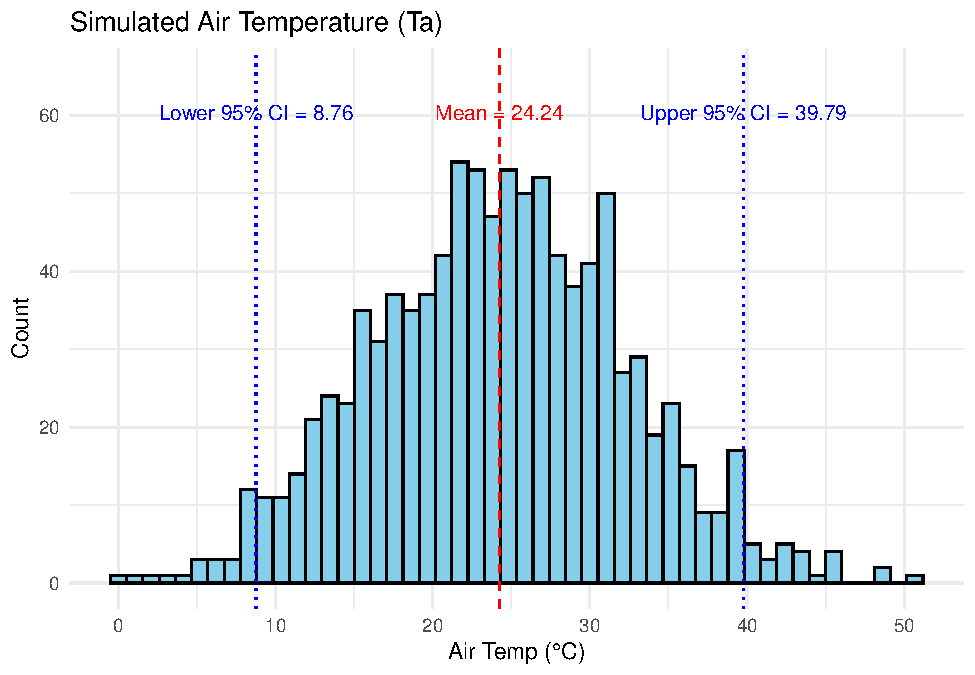
\includegraphics{V1075_MonteCarlo_Report_files/figure-latex/unnamed-chunk-5-1.pdf}

\begin{Shaded}
\begin{Highlighting}[]
\FunctionTok{ggsave}\NormalTok{(}\FunctionTok{file.path}\NormalTok{(results\_dir, }\StringTok{"Ta\_Histogram.png"}\NormalTok{))}
\end{Highlighting}
\end{Shaded}


\end{document}
